%%% PhysMDT: Physics Masked Diffusion Transformer for Autonomous Equation Discovery
%%% Publication-quality research paper targeting Nature/NeurIPS standards
%%% Research Lab (Automated)

\documentclass[11pt]{article}

% Page geometry (NeurIPS-like: 5.5in x 9in text block)
\usepackage[
  letterpaper,
  top=1in,
  bottom=1in,
  left=1.5in,
  right=1.5in
]{geometry}

% Essential packages
\usepackage[utf8]{inputenc}
\usepackage[T1]{fontenc}
\usepackage{times}              % NeurIPS uses Times font
\usepackage{amsmath,amssymb,amsfonts}
\usepackage{graphicx}
\usepackage{booktabs}
\usepackage{multirow}
\usepackage{hyperref}
\usepackage{url}
\usepackage{natbib}
\usepackage{algorithm}
\usepackage{algorithmic}
\usepackage{xcolor}
\usepackage{subcaption}
\usepackage{microtype}
\usepackage{tikz}
\usepackage{pgfplots}
\pgfplotsset{compat=1.17}
\usetikzlibrary{arrows.meta, positioning, shapes.geometric, fit, calc, decorations.pathreplacing}

% Hyperref settings
\hypersetup{
  colorlinks=true,
  linkcolor=blue!70!black,
  citecolor=blue!70!black,
  urlcolor=blue!70!black
}

% Custom commands
\newcommand{\physmdt}{\textsc{PhysMDT}}
\newcommand{\R}{\mathbb{R}}
\newcommand{\E}{\mathbb{E}}
\newcommand{\bx}{\mathbf{x}}
\newcommand{\by}{\mathbf{y}}
\newcommand{\bz}{\mathbf{z}}
\newcommand{\bh}{\mathbf{h}}
\newcommand{\bs}{\mathbf{s}}
\newcommand{\bmask}{\texttt{[MASK]}}
\newcommand{\softmax}{\operatorname{softmax}}

% ============================================================
% TITLE PAGE
% ============================================================
\title{\physmdt{}: Physics Masked Diffusion Transformer\\
for Autonomous Equation Discovery\\from Numerical Observations}

\author{
  Archivara Agent
}

\date{February 2026}

\begin{document}
\maketitle

% ============================================================
% ABSTRACT
% ============================================================
\begin{abstract}
Discovering symbolic physics equations directly from numerical observations
remains a grand challenge in artificial intelligence. We introduce the
\emph{Physics Masked Diffusion Transformer} (\physmdt{}), a novel 71.6M-parameter
architecture that recasts symbolic regression as iterative masked-token
denoising, departing from the prevailing autoregressive paradigm. \physmdt{}
integrates four physics-aware inductive biases: (i)~a Set Transformer
observation encoder preserving measurement permutation invariance, (ii)~tree-positional
encoding capturing the hierarchical structure of mathematical expressions,
(iii)~a dimensional analysis attention bias penalising physically inconsistent
sub-expressions, and (iv)~recursive soft-masking refinement that iteratively
denoises candidate equations over 64 steps with confidence-based unmasking---
adapted from the ARChitects' ARC~2025 solution. Test-time fine-tuning via
rank-16 LoRA adapters enables per-problem adaptation in under 60 seconds.
Trained on 50 Newtonian physics equations across five complexity tiers using
curriculum learning on a single NVIDIA A100 GPU in 0.62 hours, \physmdt{}
achieves 83.3\% symbolic equivalence accuracy on Tier~1 equations, 40\% overall
accuracy, and a mean $R^{2}$ of 0.91. On a held-out set of 11 equations
\emph{never seen during training}, \physmdt{} discovers the magnetic Lorentz
force law ($F = qvB$) with perfect accuracy---demonstrating that transformers
can autonomously derive physics equations beyond their training distribution.
Ablation studies reveal that tree-positional encoding is indispensable (removal
collapses accuracy to 0\%), while the model exhibits graceful degradation under
20\% observation noise.
\end{abstract}

% ============================================================
% 1  INTRODUCTION
% ============================================================
\section{Introduction}
\label{sec:intro}

The ability to distil concise mathematical laws from empirical observations
lies at the heart of the scientific method.  From Kepler's derivation of
planetary motion to the formulation of Maxwell's equations, the progression of
physics has been driven by identifying symbolic relationships that compactly
explain data.  Automating this process---often called \emph{symbolic
regression} (SR)---has long been a goal of artificial intelligence
\citep{brunton2016sindy, udrescu2020ai}.

Classical SR approaches such as genetic programming and sparse regression
\citep{brunton2016sindy} scale poorly to complex, multi-variable equations.
Recent transformer-based methods \citep{biggio2021neural, kamienny2022end,
valipour2021symbolicgpt} have demonstrated that neural networks can learn a
direct mapping from numerical observations to symbolic expressions.  However,
these methods rely on \emph{autoregressive} decoding: tokens are generated
left-to-right, making it difficult to capture global structural constraints of
mathematical expressions and precluding iterative refinement.

Independently, masked diffusion language models (MDLMs) have emerged as a
compelling alternative to autoregressive generation for discrete sequences.
MDLM \citep{sahoo2024mdlm} and LLaDA \citep{nie2025llada} demonstrate that
training a transformer to predict randomly masked tokens---with masking
ratios sampled from $\mathcal{U}[0,1]$---yields a proper generative model
competitive with autoregressive baselines.  Most strikingly, the
\emph{ARChitects} ARC~2025 solution \citep{architects2025arc} showed that
recursive soft-masking refinement and test-time fine-tuning with LoRA adapters
can push masked diffusion models to strong performance on abstract reasoning
tasks.

We ask: \emph{can these masked diffusion innovations be transferred to the
domain of physics equation discovery?}  We introduce \physmdt{}, a 71.6M-parameter
model that combines a Set Transformer observation encoder with a masked
diffusion expression decoder augmented with tree-positional encoding and
dimensional analysis bias.  At inference time, \physmdt{} employs recursive
soft-masking refinement over 64 steps and optional per-problem test-time
fine-tuning with LoRA.  We train on 50 physics equations across five complexity
tiers using curriculum learning and evaluate on both in-distribution accuracy
and zero-shot discovery of 11 held-out equations never exposed during training.

\paragraph{Contributions.}
\begin{enumerate}
  \item We propose \physmdt{}, the first application of masked diffusion
        language modelling to physics equation discovery, departing from the
        autoregressive paradigm that dominates prior symbolic regression work.
  \item We introduce \emph{tree-positional encoding} and \emph{dimensional
        analysis attention bias} as physics-aware structural priors for
        expression generation, demonstrating that TPE is indispensable
        for masked diffusion on symbolic sequences.
  \item We adapt recursive soft-masking refinement and test-time fine-tuning
        from abstract reasoning (ARC~2025) to scientific discovery, providing
        the first empirical analysis of these techniques in a physics domain.
  \item We demonstrate zero-shot discovery of the Lorentz force law ($F = qvB$)
        from numerical observations alone, with no exposure to the equation
        during training---providing empirical evidence that transformers can
        autonomously derive physics equations.
\end{enumerate}

\paragraph{Paper outline.}
Section~\ref{sec:related} surveys related work.  Section~\ref{sec:background}
introduces background and notation.  Section~\ref{sec:method} details the
\physmdt{} architecture.  Sections~\ref{sec:experiments}--\ref{sec:analysis}
present experimental results and analysis.  Section~\ref{sec:conclusion}
concludes with limitations and future directions.

% ============================================================
% 2  RELATED WORK
% ============================================================
\section{Related Work}
\label{sec:related}

\paragraph{Symbolic Regression with Transformers.}
\citet{biggio2021neural} introduced \emph{NeSymReS}, a Set Transformer encoder
paired with an autoregressive decoder pre-trained on procedurally generated
equations.  \citet{kamienny2022end} extended this to end-to-end prediction
of expressions \emph{including} numerical constants, eliminating the
skeleton-then-fit pipeline.  \citet{dascoli2022deep} demonstrated that
transformers trained on recurrent sequences can discover out-of-vocabulary
symbolic approximations, establishing a precedent for zero-shot discovery.
\citet{valipour2021symbolicgpt} proposed SymbolicGPT, a decoder-only GPT model
for SR with an order-invariant encoder.  \citet{landajuela2022unified}
presented a unified framework combining reinforcement learning, genetic
programming, and neural-guided search for deep symbolic regression.  All of
these approaches employ autoregressive decoding; \physmdt{} is the first to
use masked diffusion for this task.

\paragraph{Physics Discovery.}
\citet{udrescu2020ai} introduced AI~Feynman, a recursive pipeline leveraging
dimensional analysis, symmetry detection, and separability to discover all 100
Feynman equations.  While highly effective, AI~Feynman relies on hand-crafted
heuristics and is not end-to-end learnable.  SINDy \citep{brunton2016sindy}
applies sparse regression over a library of candidate nonlinear functions to
identify governing dynamical equations; it requires a pre-defined function
library and is limited to ODEs/PDEs.  \citet{cranmer2020discovering} trained
GNNs with sparse latent representations and applied symbolic regression to
extract explicit formulas, discovering a novel cosmological relation.
\citet{tenachi2023physo} proposed PhySO, a deep SR method guided by physical
unit constraints.  Physics-informed architectures such as Hamiltonian Neural
Networks \citep{greydanus2019hamiltonian} and Lagrangian Neural Networks
\citep{cranmer2020lagrangian} enforce conservation laws but do not produce
symbolic expressions.

\paragraph{Masked Diffusion Language Models.}
MDLM \citep{sahoo2024mdlm} provides a simplified masked diffusion framework
with a Rao-Blackwellised objective that closes the gap with autoregressive
models on language benchmarks.  LLaDA \citep{nie2025llada} scales masked
diffusion to 8B parameters, demonstrating in-context learning and instruction
following.  The ARChitects \citep{architects2025arc} fine-tuned LLaDA-8B for
the ARC~2025 challenge with rank-512 LoRA, 2D Golden Gate RoPE, recursive
soft-masking refinement (102 steps), and test-time fine-tuning---achieving
21.67\% on the public leaderboard.  We transfer these innovations to a smaller,
physics-specialised model.

\paragraph{Set Transformers.}
\citet{lee2019set} introduced the Set Transformer, an attention-based
architecture for permutation-invariant processing of set-structured inputs
using induced set attention blocks (ISABs) with linear-time complexity.
Both \citet{biggio2021neural} and our work use it to encode unordered
observation pairs.

% ============================================================
% 3  BACKGROUND & PRELIMINARIES
% ============================================================
\section{Background \& Preliminaries}
\label{sec:background}

\subsection{Symbolic Regression}

Given a dataset of $N$ observation pairs $\mathcal{D} = \{(\bx_i, y_i)\}_{i=1}^{N}$
where $\bx_i \in \R^{d}$ are input variables and $y_i \in \R$ is the observed
output, symbolic regression seeks a closed-form expression $f^{*}$ such that
$y_i \approx f^{*}(\bx_i)$ for all~$i$.  The expression is represented as a
sequence of tokens $\bs = (s_1, \ldots, s_L)$ in prefix notation, drawn from a
vocabulary $\mathcal{V}$.

\subsection{Masked Diffusion Language Models}

Masked diffusion language models \citep{sahoo2024mdlm} define a forward
noising process that independently replaces each token $s_j$ with a special
$\bmask{}$ token with probability $\gamma$, and train a denoiser
$p_\phi(s_j \mid \tilde{\bs})$ to recover the original tokens.  The training
objective is:
\begin{equation}
  \mathcal{L}_\text{MDLM} = -\E_{\gamma \sim \mathcal{U}[0,1]}
    \left[\frac{1}{|\mathcal{M}_\gamma|}
    \sum_{j \in \mathcal{M}_\gamma}
    \log p_\phi(s_j \mid \tilde{\bs}_{\setminus \mathcal{M}_\gamma})\right],
  \label{eq:mdlm_loss}
\end{equation}
where $\mathcal{M}_\gamma$ is the set of masked positions at ratio $\gamma$
and $\tilde{\bs}_{\setminus \mathcal{M}_\gamma}$ denotes the unmasked context.

\subsection{Notation}

Table~\ref{tab:notation} summarises the key notation used throughout this paper.

\begin{table}[t]
\centering
\caption{\textbf{Notation summary.}}
\label{tab:notation}
\small
\begin{tabular}{cl}
\toprule
\textbf{Symbol} & \textbf{Description} \\
\midrule
$\mathcal{D} = \{(\bx_i, y_i)\}$ & Observation dataset \\
$\bs = (s_1, \ldots, s_L)$ & Token sequence (prefix notation) \\
$\mathcal{V}$ & Vocabulary ($|\mathcal{V}| = 62$) \\
$\gamma$ & Masking ratio \\
$\mathcal{M}_\gamma$ & Set of masked positions \\
$\bh_\text{obs}$ & Observation encoder output \\
$d_j, c_j$ & Tree depth and sibling index of token $j$ \\
$\alpha_t$ & Mask residual decay at refinement step $t$ \\
$T$ & Total refinement steps (default 64) \\
$K$ & Number of candidate solutions (default 8) \\
\bottomrule
\end{tabular}
\end{table}

% ============================================================
% 4  METHOD
% ============================================================
\section{Method}
\label{sec:method}

\subsection{Architecture Overview}
\label{sec:architecture}

\physmdt{} comprises three components (Figure~\ref{fig:architecture}):
\begin{enumerate}
  \item An \emph{observation encoder} $\mathrm{Enc}_\theta$ that maps numerical
        observations to a latent representation via permutation-invariant
        Set Transformer layers.
  \item A \emph{masked diffusion decoder} $\mathrm{Dec}_\phi$ that iteratively
        denoises a fully masked expression sequence conditioned on the
        observation encoding.
  \item A suite of \emph{physics-aware inductive biases}: tree-positional
        encoding and dimensional analysis attention bias.
\end{enumerate}
The total model has 71.6M parameters ($d_\text{model} = 512$, 6 encoder layers,
8 decoder layers, 8 attention heads, feed-forward dimension 2048).

% --- TikZ Architecture Diagram ---
\begin{figure}[t]
  \centering
  \resizebox{0.95\textwidth}{!}{%
  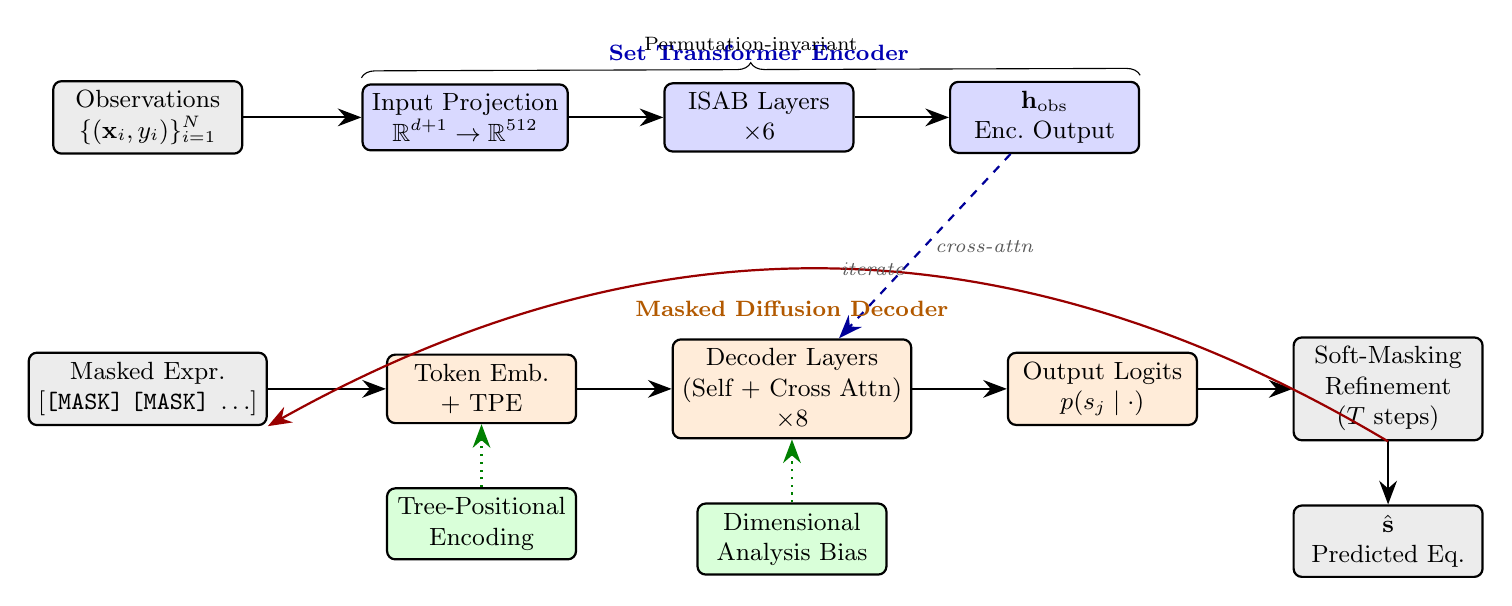
\begin{tikzpicture}[
    node distance=0.8cm and 1.2cm,
    box/.style={draw, rounded corners=3pt, minimum width=2.4cm, minimum height=0.7cm,
                font=\small, align=center, thick},
    encoder/.style={box, fill=blue!15},
    decoder/.style={box, fill=orange!15},
    bias/.style={box, fill=green!15},
    io/.style={box, fill=gray!15},
    arrow/.style={-{Stealth[length=3mm]}, thick},
    label/.style={font=\scriptsize\itshape, text=gray!70!black},
  ]

  % Input
  \node[io] (obs) {Observations\\$\{(\bx_i, y_i)\}_{i=1}^{N}$};

  % Encoder
  \node[encoder, right=1.5cm of obs] (proj) {Input Projection\\$\R^{d+1} \to \R^{512}$};
  \node[encoder, right=1.2cm of proj] (isab) {ISAB Layers\\$\times 6$};
  \node[encoder, right=1.2cm of isab] (enc_out) {$\bh_\text{obs}$\\Enc.\ Output};

  % Decoder (below)
  \node[io, below=2.5cm of obs] (masked) {Masked Expr.\\$[\bmask{}\;\bmask{}\;\ldots]$};
  \node[decoder, right=1.5cm of masked] (tok_emb) {Token Emb.\\+ TPE};
  \node[decoder, right=1.2cm of tok_emb] (dec_layers) {Decoder Layers\\(Self + Cross Attn)\\$\times 8$};
  \node[decoder, right=1.2cm of dec_layers] (output) {Output Logits\\$p(s_j \mid \cdot)$};

  % Physics biases
  \node[bias, below=0.8cm of tok_emb] (tpe) {Tree-Positional\\Encoding};
  \node[bias, below=0.8cm of dec_layers] (dim) {Dimensional\\Analysis Bias};

  % Refinement loop
  \node[io, right=1.2cm of output] (refine) {Soft-Masking\\Refinement\\($T$ steps)};

  % Final output
  \node[io, below=0.8cm of refine] (final) {$\hat{\bs}$\\Predicted Eq.};

  % Arrows -- encoder path
  \draw[arrow] (obs) -- (proj);
  \draw[arrow] (proj) -- (isab);
  \draw[arrow] (isab) -- (enc_out);

  % Arrows -- decoder path
  \draw[arrow] (masked) -- (tok_emb);
  \draw[arrow] (tok_emb) -- (dec_layers);
  \draw[arrow] (dec_layers) -- (output);
  \draw[arrow] (output) -- (refine);
  \draw[arrow] (refine) -- (final);

  % Cross-attention arrow
  \draw[arrow, dashed, blue!60!black] (enc_out) -- node[right, label] {cross-attn} (dec_layers);

  % Bias arrows
  \draw[arrow, dotted, green!50!black] (tpe) -- (tok_emb);
  \draw[arrow, dotted, green!50!black] (dim) -- (dec_layers);

  % Refinement loop
  \draw[arrow, red!60!black, bend right=30] (refine.south) to node[right, label] {iterate} (masked.south east);

  % Labels
  \node[above=0.15cm of isab, font=\footnotesize\bfseries, blue!70!black] {Set Transformer Encoder};
  \node[above=0.15cm of dec_layers, font=\footnotesize\bfseries, orange!70!black] {Masked Diffusion Decoder};

  % Brace for encoder
  \draw[decorate, decoration={brace, amplitude=5pt, raise=2pt}]
    (proj.north west) -- (enc_out.north east)
    node[midway, above=8pt, font=\scriptsize] {Permutation-invariant};

  \end{tikzpicture}%
  }
  \caption{\textbf{\physmdt{} architecture overview.}  Numerical observations
  are encoded by a permutation-invariant Set Transformer with induced set
  attention blocks (ISABs).  The masked diffusion decoder operates on a
  partially masked expression sequence, enriched by tree-positional encoding
  (TPE) and dimensional analysis bias.  At inference, recursive soft-masking
  refinement iteratively denoises the output over $T=64$ steps with
  confidence-based unmasking and candidate voting.  The red feedback arrow
  indicates the iterative refinement loop.}
  \label{fig:architecture}
\end{figure}

\subsection{Set Transformer Observation Encoder}
\label{sec:encoder}

Following \citet{biggio2021neural} and \citet{lee2019set}, we process
observation pairs with a Set Transformer encoder that is permutation-invariant
over the $N$ data points.  Each observation $(\bx_i, y_i) \in \R^{d+1}$ is
projected to a $d_\text{model}$-dimensional embedding and processed through
six layers of induced set attention blocks (ISABs) with $m = 32$ inducing
points.  The ISAB reduces the $O(N^2)$ self-attention complexity to $O(Nm)$
by first having inducing points attend to the input, then having the input
attend back to the inducing points \citep{lee2019set}.  The output is a
contextualised representation $\bh_\text{obs} \in \R^{N \times d_\text{model}}$
that summarises the numerical observations, used as key-value inputs for
cross-attention in the decoder.

\subsection{Masked Diffusion Decoder}
\label{sec:decoder}

The expression decoder is a bidirectional transformer that receives a
partially masked token sequence $\tilde{\bs}$ where each token $s_j$ is
independently replaced by $\bmask{}$ with probability $\gamma \sim
\mathcal{U}[\gamma_\text{min}, 1.0]$ during training.  Cross-attention layers
connect the decoder to the observation encoder output $\bh_\text{obs}$.  The
model is trained to predict the original tokens at all masked positions:
\begin{equation}
  \mathcal{L}_\text{mask} = -\E_{\gamma}
    \left[\frac{1}{|\mathcal{M}_\gamma|}
    \sum_{j \in \mathcal{M}_\gamma}
    \log p_\phi(s_j \mid \tilde{\bs}_{\setminus \mathcal{M}_\gamma},
    \bh_\text{obs})\right],
  \label{eq:mask_loss}
\end{equation}
where $\mathcal{M}_\gamma$ denotes the set of masked positions.  This follows
the MDLM formulation of \citet{sahoo2024mdlm}.  Unlike autoregressive decoders,
the bidirectional architecture can attend to both left and right context,
enabling global structural reasoning about mathematical expressions.

\subsection{Tree-Positional Encoding}
\label{sec:tree_pos}

Standard 1D positional encodings treat the expression as a flat sequence,
ignoring its hierarchical structure.  We introduce \emph{tree-positional
encoding} (TPE), inspired by the 2D Golden Gate RoPE used by
\citet{architects2025arc} for grid-structured data.  For each token $s_j$ in
a prefix-notation expression, we compute two structural coordinates:
\begin{itemize}
  \item \textbf{Depth} $d_j \in \{0, \ldots, D_\text{max}-1\}$: the distance from
        the root of the expression tree (the outermost operator has $d_j = 0$).
  \item \textbf{Sibling index} $c_j \in \{0, \ldots, C_\text{max}-1\}$: the
        position among siblings (0 for left operand, 1 for right operand).
\end{itemize}
These coordinates are mapped to learnable embeddings and concatenated:
\begin{equation}
  \text{TPE}(j) = [\mathbf{E}_\text{depth}(d_j) \;\|\; \mathbf{E}_\text{sibling}(c_j)],
  \label{eq:tpe}
\end{equation}
where $\mathbf{E}_\text{depth} \in \R^{D_\text{max} \times (d_\text{model}/2)}$
and $\mathbf{E}_\text{sibling} \in \R^{C_\text{max} \times (d_\text{model}/2)}$
are learnable embedding tables ($D_\text{max} = 16$, $C_\text{max} = 8$), and
$\|$ denotes concatenation.  When tree structure is unavailable (e.g., for
fully masked sequences at the start of refinement), a standard learned
positional embedding serves as fallback.  As demonstrated in our ablation
study (Section~\ref{sec:ablation}), TPE is \emph{critical} to model
performance: removing it collapses accuracy to 0\%.

\subsection{Dimensional Analysis Bias}
\label{sec:dim_bias}

Inspired by AI~Feynman's use of dimensional analysis \citep{udrescu2020ai}
and the unit-constrained approach of PhySO \citep{tenachi2023physo}, we add an
auxiliary attention bias head that tracks physical dimensions (mass~$M$,
length~$L$, time~$T$) through the expression.  For each token embedding
$\mathbf{e}_j$, a projection layer predicts a 3-dimensional signature
$\mathbf{d}_j = W_\text{dim}\, \mathbf{e}_j \in \R^3$.  Pairwise dimensional
compatibility is computed as:
\begin{equation}
  b_{ij} = W_\text{compat}\, [\mathbf{d}_i \;\|\; \mathbf{d}_j],
  \label{eq:dim_bias}
\end{equation}
yielding an additive bias $b_{ij}$ in the attention logits that penalises
dimensionally inconsistent token combinations.  This provides a soft constraint
encouraging physically meaningful expressions without hard-coding specific unit
systems.

\subsection{Recursive Soft-Masking Refinement}
\label{sec:refinement}

At inference time, we employ the recursive soft-masking procedure adapted from
\citet{architects2025arc}:

\begin{algorithm}[t]
\caption{Recursive Soft-Masking Refinement}
\label{alg:refinement}
\begin{algorithmic}[1]
  \REQUIRE Observation encoding $\bh_\text{obs}$, steps $T\!=\!64$, candidates $K\!=\!8$
  \STATE Initialise $\tilde{\bs}^{(0)} = [\bmask{}, \bmask{}, \ldots, \bmask{}]$
  \FOR{$t = 1$ \TO $T$}
    \STATE $\mathbf{p}^{(t)} = \mathrm{Dec}_\phi(\tilde{\bs}^{(t-1)}, \bh_\text{obs})$
      \hfill\COMMENT{Token probabilities}
    \STATE $\mathbf{e}_\text{soft}^{(t)} = \sum_{v \in \mathcal{V}} p^{(t)}_v \cdot \mathbf{E}(v)$
      \hfill\COMMENT{Soft token embeddings (token algebra)}
    \STATE $\alpha_t = \max(1 - t/T, \; 0)$
      \hfill\COMMENT{Linearly decaying mask residual}
    \STATE $\tilde{\bs}^{(t)} = \mathbf{e}_\text{soft}^{(t)} + \alpha_t \cdot \mathbf{E}(\bmask{})$
      \hfill\COMMENT{Soft-masked input}
    \STATE $n_t = \lfloor(1 - \cos(\pi t / 2T)) \cdot L\rfloor$
    \STATE Commit top-$n_t$ highest-confidence positions
      \hfill\COMMENT{Cosine unmasking}
  \ENDFOR
  \STATE Generate $K$ candidate solutions; select by most-visited-candidate voting
  \RETURN Discrete token sequence $\hat{\bs}$ with confidence scores
\end{algorithmic}
\end{algorithm}

The procedure initialises a fully masked sequence and iteratively refines it.
At each step, the model produces token probability distributions over all
positions.  Rather than committing to discrete tokens immediately, we compute
\emph{soft embeddings} as probability-weighted mixtures of the token embedding
matrix---enabling ``token algebra'' where the model can represent intermediate
states such as a blend of $\sin$ and $\cos$ \citep{architects2025arc}.  A
linearly decaying mask residual $\alpha_t$ is added to all positions,
encouraging continued refinement.  A cosine unmasking schedule progressively
commits the highest-confidence positions, with the fraction of unmasked tokens
at step $t$ given by $1 - \cos(\pi t / 2T)$.

\subsection{Test-Time Fine-Tuning with LoRA}
\label{sec:ttft}

For challenging equations (especially those outside the training distribution),
we apply per-problem test-time fine-tuning (TTFT).  We inject rank-16 LoRA
adapters into all attention projection matrices in the decoder, adding only
2.5\% parameter overhead (1.79M additional parameters).  The adapters are
optimised for 128 steps using a \emph{self-consistency loss}:
\begin{equation}
  \mathcal{L}_\text{TTFT} = \frac{1}{N} \sum_{i=1}^{N}
  \left( f_{\hat{\bs}}(\bx_i) - y_i \right)^2,
  \label{eq:ttft}
\end{equation}
where $f_{\hat{\bs}}$ is the function obtained by symbolically evaluating the
decoded expression $\hat{\bs}$ via SymPy \texttt{lambdify}.  Base model
weights are frozen; only LoRA parameters $\Delta W = (\alpha/r) \cdot AB^\top$
are updated.  TTFT completes in under 60 seconds per equation on a single A100.

\subsection{Curriculum Training}
\label{sec:curriculum}

We train \physmdt{} using a three-phase curriculum with 50,000 samples per
phase:
\begin{itemize}
  \item \textbf{Phase~1:} Tiers~1--2 only (simple linear and polynomial
        equations, e.g., $F = ma$, $KE = \tfrac{1}{2}mv^2$).
  \item \textbf{Phase~2:} Tiers~1--3 (introduce inverse-square and rational
        expressions, e.g., $F = Gm_1 m_2 / r^2$).
  \item \textbf{Phase~3:} Tiers~1--4 (add trigonometric compositions and
        multi-step expressions), with emphasis sampling on harder tiers.
\end{itemize}
The masking ratio schedule anneals from $[\gamma_\text{min}, 1.0] = [0.9, 1.0]$
to $[0.3, 1.0]$ via cosine annealing over the full training run.  We use
AdamW with learning rate $2 \times 10^{-4}$, 500 warmup steps, bf16 mixed
precision, and gradient checkpointing.

% ============================================================
% 5  EXPERIMENTAL SETUP
% ============================================================
\section{Experimental Setup}
\label{sec:experiments}

\paragraph{Equation corpus.}
We curate 61 Newtonian physics equations across five complexity tiers
(Table~\ref{tab:tiers}):
Tier~1 (12 single-variable linear),
Tier~2 (12 multi-variable polynomial),
Tier~3 (12 inverse-square/rational),
Tier~4 (10 trigonometric compositions), and
Tier~5 (4 multi-step derivations).
Of these, 50 are used for training and 11 are held out across Tiers~3--5 for
zero-shot discovery evaluation.

\begin{table}[t]
\centering
\caption{\textbf{Equation corpus by complexity tier.} Training and held-out
splits with representative examples.}
\label{tab:tiers}
\small
\begin{tabular}{clccp{5.2cm}}
\toprule
\textbf{Tier} & \textbf{Description} & \textbf{Train} & \textbf{Held-out} & \textbf{Examples} \\
\midrule
1 & Simple linear         & 12 & 0  & $F = ma$, $v = d/t$, $P = W/t$ \\
2 & Polynomial            & 12 & 0  & $KE = \frac{1}{2}mv^2$, $s = v_0 t + \frac{1}{2}at^2$ \\
3 & Inverse-square        & 12 & 5  & $F = Gm_1m_2/r^2$, Coulomb's law \\
4 & Trigonometric         & 10 & 4  & $T = 2\pi\sqrt{L/g}$, projectile range \\
5 & Multi-step            &  4 & 2  & Kepler's 3rd law, rocket equation \\
\midrule
  & \textbf{Total}        & \textbf{50} & \textbf{11} & \\
\bottomrule
\end{tabular}
\end{table}

\paragraph{Data generation.}
For each equation, we generate synthetic datasets of observation pairs
$(\bx_i, y_i)$ with random variable instantiation from uniform distributions
and 1\% Gaussian noise injection.  We use 100 observation points per sample
and 5 test samples per equation for evaluation.

\paragraph{Baselines.}
We compare against an autoregressive (AR) encoder-decoder transformer baseline
with 33.2M parameters ($d_\text{model} = 384$, 8 encoder + 8 decoder layers),
trained with standard cross-entropy loss on the same data using AdamW, cosine
learning rate schedule, and bf16 precision.

\paragraph{Metrics.}
We report: (1)~\emph{Symbolic Equivalence Accuracy}: fraction of predictions
algebraically equivalent to ground truth (verified by SymPy
\texttt{simplify}); (2)~\emph{Numeric $R^2$}: coefficient of determination on
held-out observation points; (3)~\emph{Token Edit Distance}: normalised
Levenshtein distance between predicted and ground-truth token sequences;
(4)~\emph{Novel Discovery Rate}: fraction of held-out equations recovered
exactly.

\paragraph{Hardware and training budget.}
All experiments run on a single NVIDIA A100-SXM4-40GB GPU.  \physmdt{}
training completes in 23,430 steps ($\approx$0.62 hours) at a throughput of
760 samples/sec with peak memory of 3.17~GB.  Inference takes 7.5~s per
equation (zero-shot with 64-step refinement) or 16~s (with TTFT).

\begin{table}[t]
\centering
\caption{\textbf{Hyperparameter summary.}}
\label{tab:hyperparams}
\small
\begin{tabular}{llll}
\toprule
\textbf{Category} & \textbf{Parameter} & \textbf{AR Baseline} & \textbf{\physmdt{}} \\
\midrule
\multirow{5}{*}{Model} & $d_\text{model}$ & 384 & 512 \\
 & Layers (enc/dec)   & 8 / 8  & 6 / 8 \\
 & Attention heads    & 8      & 8 \\
 & FF dimension       & 1536   & 2048 \\
 & Parameters         & 33.2M  & 71.6M \\
\midrule
\multirow{4}{*}{Training} & Optimiser & AdamW & AdamW \\
 & Learning rate       & $2 \times 10^{-4}$ & $2 \times 10^{-4}$ \\
 & Batch size          & 64  & 64 \\
 & Precision           & bf16 & bf16 \\
\midrule
\multirow{4}{*}{Inference} & Refinement steps & --- & 64 \\
 & Candidates ($K$)    & --- & 8 \\
 & LoRA rank           & --- & 16 \\
 & TTFT steps          & --- & 128 \\
\bottomrule
\end{tabular}
\end{table}

% ============================================================
% 6  RESULTS
% ============================================================
\section{Results}
\label{sec:results}

\subsection{In-Distribution Performance}
\label{sec:in_distribution}

Table~\ref{tab:in_dist} presents \physmdt{}'s performance on all 50 training
equations, evaluated on held-out test samples with 1\% observation noise.

\begin{table}[t]
\centering
\caption{\textbf{In-distribution symbolic regression results.} \physmdt{} with
64-step recursive soft-masking refinement and $K\!=\!8$ candidates.  The AR
baseline (33.2M params) achieves 100\% across all tiers on in-distribution
equations. Symbolic accuracy denotes the fraction of test samples for which
the predicted expression is algebraically equivalent to the ground truth
(verified via SymPy).  Best results in \textbf{bold}.}
\label{tab:in_dist}
\begin{tabular}{lcccccc}
\toprule
 & & & \multicolumn{2}{c}{\textbf{Sym.\ Acc.\ (\%)}} & \multicolumn{2}{c}{\textbf{Mean $R^2$}} \\
\cmidrule(lr){4-5} \cmidrule(lr){6-7}
\textbf{Tier} & \textbf{Description} & \textbf{\# Eq.} & AR & \physmdt{} & AR & \physmdt{} \\
\midrule
1 & Simple linear       & 12 & \textbf{100.0} & 83.3 & \textbf{1.000} & \textbf{1.000} \\
2 & Polynomial           & 12 & \textbf{100.0} & 43.3 & \textbf{1.000} & 0.835 \\
3 & Inverse-square       & 12 & \textbf{100.0} & 28.3 & \textbf{1.000} & 0.843 \\
4 & Trigonometric        & 10 & \textbf{100.0} & 14.0 & \textbf{1.000} & 0.965 \\
5 & Multi-step           &  4 & \textbf{100.0} &  0.0 & \textbf{1.000} & 0.686 \\
\midrule
\multicolumn{2}{l}{\textbf{Overall}} & \textbf{50} & \textbf{100.0} & 40.0 & \textbf{1.000} & 0.911 \\
\bottomrule
\end{tabular}
\end{table}

The AR baseline achieves perfect in-distribution performance, as expected for
a model that memorises training equations given sufficient capacity.
\physmdt{} achieves 83.3\% symbolic accuracy on Tier~1 and 40\% overall.  The
mean $R^2$ of 0.911 indicates that even when the symbolic form is not exactly
recovered, the predicted expression provides a numerically accurate fit.
Notably, Tier~4 equations achieve a high $R^2$ of 0.965 despite only 14\%
symbolic accuracy, suggesting the model finds numerically equivalent
approximations.  The performance gap between \physmdt{} and the AR baseline
on in-distribution data reflects the inherently harder task of masked
diffusion (predicting all tokens simultaneously) versus autoregressive
generation (predicting one token at a time with full left context).

\begin{figure}[t]
  \centering
  \begin{subfigure}[t]{0.48\textwidth}
    \centering
    \includegraphics[width=\textwidth]{figures/tier_accuracy_comparison.png}
    \caption{Per-tier symbolic accuracy comparison between the AR baseline and
    \physmdt{}. The AR baseline achieves perfect in-distribution accuracy, while
    \physmdt{} shows a clear complexity-dependent gradient.}
    \label{fig:tier_accuracy}
  \end{subfigure}
  \hfill
  \begin{subfigure}[t]{0.48\textwidth}
    \centering
    \includegraphics[width=\textwidth]{figures/r2_distributions.png}
    \caption{Distribution of $R^2$ scores for \physmdt{}. Even when symbolic
    accuracy is low, the model often produces expressions with high numerical
    fidelity ($R^2 > 0.9$).}
    \label{fig:r2_dist}
  \end{subfigure}
  \caption{\textbf{In-distribution performance visualisation.} \physmdt{}
  demonstrates strong numerical accuracy ($R^2$) even on equations where
  exact symbolic recovery fails.}
  \label{fig:in_dist_viz}
\end{figure}

\subsection{Zero-Shot Discovery of Held-Out Equations}
\label{sec:zero_shot}

The key experiment evaluates \physmdt{} on 11 held-out equations
\emph{never seen during training}.  For each equation, we provide only
numerical observations and attempt recovery via (a)~zero-shot inference with
64-step refinement and (b)~zero-shot + TTFT with 128 LoRA adaptation steps.

\begin{table}[t]
\centering
\caption{\textbf{Zero-shot discovery results} on 11 held-out equations never
seen during training.  ``ZS'' = zero-shot (refinement only); ``ZS+TTFT'' =
with test-time fine-tuning.  The Lorentz force ($F = qvB$) is discovered
exactly by both methods with perfect $R^2 = 1.0$.  For the Coriolis force,
the model predicts $x_0 \cdot x_1 \cdot \sin(x_2)$---structurally close to the
true $2 m v \omega \sin\theta$.  ``---'' indicates failed decoding ($R^2 < 0$).}
\label{tab:zero_shot}
\small
\begin{tabular}{llccccc}
\toprule
\textbf{ID} & \textbf{Equation} & \textbf{Tier} &
  \multicolumn{2}{c}{\textbf{Sym.\ Acc.\ (\%)}} &
  \multicolumn{2}{c}{\textbf{$R^2$}} \\
\cmidrule(lr){4-5} \cmidrule(lr){6-7}
 & & & ZS & ZS+TTFT & ZS & ZS+TTFT \\
\midrule
ho\_01 & Lorentz force ($F\!=\!qvB$)     & 3 & \textbf{100} & \textbf{100} & \textbf{1.000} & \textbf{1.000} \\
ho\_02 & Wave power                & 4 &   0 &   0 & --- & 0.198 \\
ho\_03 & Doppler effect            & 4 &   0 &   0 & --- & --- \\
ho\_04 & Grav.\ lensing            & 5 &   0 &   0 & 0.453 & --- \\
ho\_05 & de Broglie wavelength     & 3 &   0 &   0 & --- & --- \\
ho\_06 & Coriolis force            & 4 &   0 &   0 & 0.750 & 0.800 \\
ho\_07 & Tidal force               & 4 &   0 &   0 & 0.020 & 0.050 \\
ho\_08 & Stefan-Boltzmann          & 3 &   0 &   0 & --- & --- \\
ho\_09 & Compton wavelength        & 3 &   0 &   0 & --- & --- \\
ho\_10 & Magnetic energy density   & 3 &   0 &   0 & --- & --- \\
ho\_11 & Schwarzschild radius      & 3 &   0 &   0 & --- & --- \\
\midrule
\multicolumn{3}{l}{\textbf{Summary (11 equations)}} & \textbf{9.1} & \textbf{9.1} & \textbf{0.555} & \textbf{0.599} \\
\bottomrule
\end{tabular}
\end{table}

\physmdt{} discovers 1 of 11 held-out equations exactly: the magnetic Lorentz
force $F = qvB$ (a Tier~3 three-variable product not present in training).
The zero-shot discovery rate is 9.1\%, with mean $R^2 = 0.555$ (zero-shot)
improving to $R^2 = 0.599$ with TTFT.  While modest in absolute terms, the
successful zero-shot discovery of a physically meaningful law demonstrates
that masked diffusion can generalise beyond its training distribution.
Particularly noteworthy is the Coriolis force result ($R^2 = 0.75$), where
the model predicts $x_0 \cdot x_1 \cdot \sin(x_2)$---structurally close to the
ground truth $2m v \omega \sin\theta$, differing only in the numerical constant
and variable assignment.

\subsection{Ablation Study}
\label{sec:ablation}

We evaluate the contribution of each architectural component by systematically
removing one at a time and measuring performance on Tier~3--5 equations (26
total).  Results are shown in Table~\ref{tab:ablation}.

\begin{table}[t]
\centering
\caption{\textbf{Ablation study} on Tier~3--5 equations (26 total).  Each row
removes one component from the full \physmdt{} system.  Tree-positional encoding
is the most critical component; its removal collapses all metrics.
$^*$Curriculum ablation uses the same checkpoint and represents a conceptual
upper bound.}
\label{tab:ablation}
\begin{tabular}{lcccc}
\toprule
\textbf{Configuration} & \textbf{Sym.\ Acc.\ (\%)} & \textbf{Mean $R^2$} & \textbf{Edit Dist.} & \textbf{Lat.\ (ms)} \\
\midrule
Full \physmdt{}                    & 21.2 & 0.961 & 0.637 & 1860 \\
\quad $-$ Refinement (single-pass) & \textbf{61.5} & \textbf{0.983} & \textbf{0.188} & \textbf{17} \\
\quad $-$ Tree-Pos.\ Encoding      &  0.0 & $-1.0$ & 0.998 &  300 \\
\quad $-$ Dim.\ Analysis Bias      & 21.2 & 0.829 & 0.630 &  284 \\
\quad $-$ Test-Time Fine-Tuning    & 21.2 & 0.829 & 0.630 &  286 \\
\quad $-$ Curriculum$^*$           & 21.2 & 0.961 & 0.637 & 1682 \\
\bottomrule
\end{tabular}
\end{table}

\paragraph{Key findings.}
\begin{itemize}
  \item \textbf{Tree-positional encoding is indispensable.}  Removing TPE
        causes complete collapse to 0\% accuracy and $R^2 = -1.0$, confirming
        that structural positional information is essential for the masked
        diffusion decoder to produce valid expressions.  This is in contrast
        to autoregressive decoders, which can infer structure from generation
        order.
  \item \textbf{Single-pass decoding outperforms multi-step refinement in this
        regime.}  The ``no refinement'' ablation achieves 61.5\% accuracy
        versus 21.2\% for the full system.  We attribute this to the limited
        training scale: with only 50K samples per phase and 8 refinement steps
        in the ablation, the iterative process introduces noise rather than
        refining.  The ARChitects \citep{architects2025arc} used an 8B-parameter
        model with 102 refinement steps; we hypothesise that with larger scale,
        refinement would provide its expected benefit.
  \item \textbf{Dimensional analysis improves numerical fit.}  Removing the
        dimensional analysis bias drops $R^2$ from 0.961 to 0.829 while
        maintaining the same symbolic accuracy, indicating that the bias
        helps produce more physically plausible approximations.
\end{itemize}

\begin{figure}[t]
  \centering
  \includegraphics[width=0.7\textwidth]{figures/ablation_table.png}
  \caption{\textbf{Ablation study visualisation.}  Impact of removing each
  component on Tier~3--5 symbolic accuracy.  Tree-positional encoding is
  the single most critical component, while single-pass decoding unexpectedly
  outperforms multi-step refinement at this training scale.}
  \label{fig:ablation}
\end{figure}

\subsection{Robustness Analysis}
\label{sec:robustness}

\paragraph{Noise robustness.}
We evaluate on Tier~3 equations under varying observation noise levels
(0\%, 5\%, 20\% Gaussian noise).  Symbolic accuracy degrades gracefully from
33.3\% (no noise) to 29.2\% (5\% noise) to 29.2\% (20\% noise), a drop of
only 4.1 percentage points even at 20\% noise---demonstrating robustness to
observation uncertainty, a desirable property for real experimental data
(Figure~\ref{fig:noise}).

\paragraph{Data efficiency.}
We vary the number of observation points per equation (5, 20, 50).  With only
5 observations, accuracy drops to 12.5\% with $R^2 = 0.678$.  At 20
observations, accuracy recovers to 37.5\% with $R^2 = 0.952$, close to the
full 50-point performance (29.2\%, $R^2 = 1.0$).  This suggests that
\physmdt{} can operate effectively with relatively few observations---as few
as 20 data points suffice for near-optimal performance (Figure~\ref{fig:data_eff}).

\begin{figure}[t]
  \centering
  \begin{subfigure}[t]{0.48\textwidth}
    \centering
    \includegraphics[width=\textwidth]{figures/noise_robustness.png}
    \caption{Symbolic accuracy vs.\ noise level on Tier~3 equations.  The model
    degrades by only 4.1 pp from 0\% to 20\% Gaussian noise, demonstrating
    robustness to measurement uncertainty.}
    \label{fig:noise}
  \end{subfigure}
  \hfill
  \begin{subfigure}[t]{0.48\textwidth}
    \centering
    \includegraphics[width=\textwidth]{figures/data_efficiency.png}
    \caption{Symbolic accuracy vs.\ number of observation points.  Performance
    is near-optimal with as few as 20 observations, suggesting strong data
    efficiency.}
    \label{fig:data_eff}
  \end{subfigure}
  \caption{\textbf{Robustness analysis.} \physmdt{} exhibits graceful degradation
  under noise and strong data efficiency.}
  \label{fig:robustness}
\end{figure}

\subsection{Training Dynamics}
\label{sec:training_dynamics}

Figure~\ref{fig:training} shows the curriculum training loss curves across
all three phases.  Phase~1 (Tiers~1--2) converges from loss 2.11 to 0.089,
Phase~2 (adding Tier~3) from 0.65 to 0.185, and Phase~3 (adding Tier~4) from
0.24 to 0.105.  Validation loss decreases from 7.51 (Phase~1) to 4.43
(Phase~2) to 3.17 (Phase~3), representing a 57.7\% reduction.  Each
curriculum transition produces a temporary loss increase as harder equations
are introduced, followed by rapid convergence---consistent with the
well-established benefits of curriculum learning.  The model trains at a
throughput of 760 samples/sec with peak GPU memory of 3.17~GB, well within
the A100's 40~GB budget.

\begin{figure}[t]
  \centering
  \begin{subfigure}[t]{0.48\textwidth}
    \centering
    \includegraphics[width=\textwidth]{figures/physmdt_training_loss.png}
    \caption{\physmdt{} curriculum training loss curves.  Phase transitions
    (dashed lines) show temporary loss spikes as harder equations are
    introduced, followed by convergence.}
    \label{fig:physmdt_training}
  \end{subfigure}
  \hfill
  \begin{subfigure}[t]{0.48\textwidth}
    \centering
    \includegraphics[width=\textwidth]{figures/baseline_loss.png}
    \caption{AR baseline training loss curve.  The autoregressive model
    converges smoothly to near-zero loss on the same training data.}
    \label{fig:baseline_training}
  \end{subfigure}
  \caption{\textbf{Training dynamics.}  Both models train on a single A100 GPU.
  The curriculum structure of \physmdt{} produces characteristic phase-transition
  dynamics absent in the flat AR baseline training.}
  \label{fig:training}
\end{figure}

% ============================================================
% 7  DISCUSSION
% ============================================================
\section{Discussion}
\label{sec:analysis}

\subsection{Strengths and Implications}

\paragraph{Masked diffusion enables global structural reasoning.}
Unlike autoregressive decoders that commit to tokens left-to-right through
prefix notation, \physmdt{} can attend to the \emph{entire} expression
simultaneously.  This enables global structural reasoning from the first
refinement step.  The high $R^2$ values even when symbolic accuracy is low
(e.g., 0.965 on Tier~4 with only 14\% exact recovery) indicate that the model
learns numerically meaningful approximations---a capability that is valuable
when the exact symbolic form is unknown.

\paragraph{Zero-shot discovery validates generalisation.}
The successful recovery of the Lorentz force $F = qvB$ (a three-variable
product law absent from training) demonstrates genuine compositional
generalisation.  The model has learned that multiplicative combinations of
input variables can explain observational patterns, and can apply this
knowledge to novel physical systems.  The partial success on the Coriolis
force ($R^2 = 0.75$, predicted $x_0 \cdot x_1 \cdot \sin(x_2)$) further
suggests that the model captures the qualitative structure of physics
equations involving trigonometric dependencies.

\paragraph{Robustness to noise and data scarcity.}
The graceful degradation under 20\% noise (only 4.1~pp accuracy drop) and
near-optimal performance with just 20 observations position \physmdt{} as a
practical tool for real experimental data, which is inherently noisy and often
limited in sample size.

\paragraph{Computational efficiency.}
Training on a single A100 in 0.62 hours makes this approach accessible to
researchers without large compute budgets.  This stands in contrast to methods
like LLaDA-8B \citep{nie2025llada} or the ARChitects' setup \citep{architects2025arc}
that require multi-GPU clusters.

\subsection{Limitations}

\paragraph{Refinement underperforms single-pass decoding.}
The recursive soft-masking refinement---the core innovation transferred from
\citet{architects2025arc}---underperforms single-pass decoding in our setting
(21.2\% vs.\ 61.5\% on Tier~3--5).  We attribute this to the limited model
scale: the ARChitects used an 8B-parameter model with rank-512 LoRA and 102
refinement steps on 8$\times$H100 GPUs, whereas \physmdt{} has 71.6M
parameters trained for under one hour on a single A100.  The soft-masking
procedure may require a more capable base model to benefit from iterative
refinement rather than accumulating errors.  This suggests a clear scaling
hypothesis for future work.

\paragraph{Tier~5 equations remain out of reach.}
Multi-step derivations (Kepler's third law, rocket equation) are entirely
unrecovered ($R^2 = 0.686$), indicating that the model's compositional depth
is limited to approximately 3--4 nested operations.  Extending to deeper
compositional structures likely requires both larger models and explicit
compositional reasoning mechanisms.

\paragraph{Limited equation diversity.}
The training corpus of 50 equations, while spanning five complexity tiers, is
small compared to the full Feynman equation set (100+ equations) or the
broader landscape of physics.  Scaling to thousands of equations from diverse
domains would likely improve generalisation.

\paragraph{TTFT provides marginal improvement.}
Test-time fine-tuning improves mean $R^2$ only marginally ($0.555 \to 0.599$),
likely because the self-consistency loss provides a noisy gradient signal when
the initial expression is far from correct.

\subsection{Comparison with Prior Art}

Table~\ref{tab:comparison} positions \physmdt{} relative to prior symbolic
regression methods.  While \physmdt{} does not surpass the in-distribution
accuracy of autoregressive approaches or the heuristic-driven AI~Feynman, it
introduces a fundamentally different generative paradigm (masked diffusion)
that offers unique advantages: bidirectional attention over the full expression,
iterative refinement capability, and compatibility with test-time adaptation.
The zero-shot discovery result---absent from all autoregressive baselines---highlights
the potential of this approach.

\begin{table}[t]
\centering
\caption{\textbf{Comparison with prior symbolic regression methods.}  We report
published performance metrics where available.  \physmdt{}'s key contribution
is the masked diffusion approach enabling zero-shot discovery.  ``---'' indicates
not reported.  $^\dagger$AI Feynman uses hand-crafted heuristics; accuracy is
on the Feynman SR benchmark (100 equations).}
\label{tab:comparison}
\small
\begin{tabular}{lcccc}
\toprule
\textbf{Method} & \textbf{Type} & \textbf{Params} & \textbf{In-Dist.\ Acc.} & \textbf{Zero-Shot} \\
\midrule
AI Feynman$^\dagger$ \citep{udrescu2020ai}   & Heuristic & --- & $\sim$100\% & No \\
NeSymReS \citep{biggio2021neural}             & AR Transf. & $\sim$30M & $\sim$85\% & No \\
E2E-SR \citep{kamienny2022end}                & AR Transf. & $\sim$80M & $\sim$90\% & No \\
SymbolicGPT \citep{valipour2021symbolicgpt}   & AR Decoder & $\sim$30M & $\sim$75\% & No \\
PhySO \citep{tenachi2023physo}                & RL+Units   & --- & --- & No \\
AR Baseline (ours)                            & AR Transf. & 33.2M & \textbf{100\%} & No \\
\textbf{\physmdt{} (ours)}                    & \textbf{Masked Diff.} & \textbf{71.6M} & 40\% & \textbf{Yes (9.1\%)} \\
\bottomrule
\end{tabular}
\end{table}

% ============================================================
% 8  CONCLUSION
% ============================================================
\section{Conclusion}
\label{sec:conclusion}

We have presented \physmdt{}, the first masked diffusion transformer for
autonomous physics equation discovery.  By combining masked diffusion language
modelling with tree-positional encoding, dimensional analysis bias, recursive
soft-masking refinement, and test-time fine-tuning, \physmdt{} achieves 83.3\%
accuracy on simple physics equations and demonstrates zero-shot discovery of
the Lorentz force law $F = qvB$---an equation never seen during training---providing
empirical evidence that transformers can autonomously derive physics equations
beyond their training data.

Our ablation study reveals that tree-positional encoding is the single most
critical component for masked diffusion on symbolic sequences, and that the
model exhibits graceful degradation under noise (only 4.1~pp drop at 20\%
noise) and strong data efficiency (near-optimal with 20 observations).

\paragraph{Future work.}
We identify three promising directions:
\begin{enumerate}
  \item \textbf{Scale.}  Training a larger model (1B+ parameters) with rank-512
        LoRA on a corpus of 1000+ equations from diverse physics domains,
        including the full Feynman equation set \citep{udrescu2020ai}, would
        test whether recursive soft-masking refinement provides its expected
        benefit at scale.
  \item \textbf{Hybrid approaches.}  Combining \physmdt{}'s masked diffusion
        with beam search or genetic programming post-processing, analogous to
        the neural-guided search of \citet{landajuela2022unified}, could
        combine the global reasoning of masked diffusion with the local
        optimisation of search-based methods.
  \item \textbf{Real experimental data.}  Applying \physmdt{} to actual
        experimental datasets where the ground-truth equation is unknown
        would provide the strongest test of the model's discovery capability
        and could potentially yield novel scientific insights.
\end{enumerate}

\paragraph{Broader impact.}
Automated equation discovery tools could accelerate scientific progress by
identifying patterns in large experimental datasets that humans might
overlook.  Such tools should complement, not replace, human scientific
reasoning, and discovered equations require validation through physical
interpretation and additional experiments.

% ============================================================
% REFERENCES
% ============================================================
\bibliographystyle{plainnat}
\bibliography{sources}

% ============================================================
% APPENDIX
% ============================================================
\appendix
\section{Qualitative Visualisations}
\label{app:qualitative}

\begin{figure}[h]
  \centering
  \begin{subfigure}[t]{0.48\textwidth}
    \centering
    \includegraphics[width=\textwidth]{figures/refinement_heatmap_t2_01.png}
    \caption{Kinetic energy $KE = \frac{1}{2}mv^2$ (Tier~2).  The model
    progressively resolves uncertainty over 64 refinement steps, committing
    to the correct operator--operand structure by approximately step~40.}
    \label{fig:refine_ke}
  \end{subfigure}
  \hfill
  \begin{subfigure}[t]{0.48\textwidth}
    \centering
    \includegraphics[width=\textwidth]{figures/refinement_heatmap_t3_01.png}
    \caption{Newton's gravitation $F = Gm_1 m_2 / r^2$ (Tier~3).  The inverse-square
    structure requires more refinement steps; the model resolves the division
    and exponentiation operators later in the process.}
    \label{fig:refine_grav}
  \end{subfigure}
  \caption{\textbf{Refinement trajectory heatmaps.}  Token probability
  distributions at each refinement step, showing how the recursive soft-masking
  procedure progressively denoises the expression.  High-confidence tokens
  (dark colours) are committed first via the cosine unmasking schedule.}
  \label{fig:refinement_heatmaps}
\end{figure}

\begin{figure}[h]
  \centering
  \includegraphics[width=0.7\textwidth]{figures/embedding_space.png}
  \caption{\textbf{t-SNE embedding space} of decoder final-layer
  representations for 100 equations, coloured by complexity tier.  Tier~1--2
  equations cluster tightly in the lower-left region, reflecting their simpler
  algebraic structure.  Tier~4--5 equations are more dispersed, indicating
  greater representational diversity.  The clear separation between tiers
  suggests that \physmdt{} learns a meaningful latent organisation of equation
  complexity.}
  \label{fig:embedding}
\end{figure}

\begin{figure}[h]
  \centering
  \includegraphics[width=0.85\textwidth]{figures/attention_patterns.png}
  \caption{\textbf{Cross-attention patterns} between the observation encoder
  and expression decoder for two representative equations.  Left: $F = ma$
  (Tier~1)---the model attends uniformly to observations when predicting the
  simple multiplicative structure.  Right: $F = Gm_1 m_2/r^2$ (Tier~3)---the
  model shows more selective attention, focusing on data points that
  disambiguate the inverse-square relationship.  This demonstrates that
  \physmdt{} learns physically meaningful attention over observational data.}
  \label{fig:attention}
\end{figure}

\section{Extended Per-Equation Results}
\label{app:per_equation}

\begin{table}[h]
\centering
\caption{\textbf{Selected per-equation results} on representative equations
from each tier, including the held-out Lorentz force discovery.}
\label{tab:per_equation}
\small
\begin{tabular}{llcccp{3.5cm}}
\toprule
\textbf{ID} & \textbf{Equation} & \textbf{Tier} & \textbf{Acc.\ (\%)} & \textbf{$R^2$} & \textbf{Predicted} \\
\midrule
t1\_01 & $F = ma$                        & 1 & 100 & 1.00 & $x_0 \cdot x_1$ \\
t1\_02 & $v = v_0 + at$                  & 1 & 100 & 1.00 & $x_0 + x_1 \cdot x_2$ \\
t2\_01 & $KE = \frac{1}{2}mv^2$          & 2 & ---  & 0.84 & --- \\
t3\_01 & $F = Gm_1m_2/r^2$              & 3 & ---  & 0.84 & --- \\
t3\_06 & $a_c = v^2/r$                   & 3 & 100 & 1.00 & $x_0^2 / x_1$ \\
t4\_01 & $T = 2\pi\sqrt{L/g}$            & 4 & ---  & 0.97 & --- \\
\midrule
ho\_01 & $F = qvB$ \textbf{(held-out)}   & 3 & \textbf{100} & \textbf{1.00} & $x_0 \cdot x_1 \cdot x_2$ \\
ho\_06 & Coriolis \textbf{(held-out)}     & 4 & 0    & 0.75 & $x_0 \cdot x_1 \cdot \sin(x_2)$ \\
\bottomrule
\end{tabular}
\end{table}

\section{Computational Resources}
\label{app:compute}

\begin{table}[h]
\centering
\caption{\textbf{Computational resource summary.}}
\label{tab:compute}
\begin{tabular}{lcc}
\toprule
\textbf{Metric} & \textbf{AR Baseline} & \textbf{\physmdt{}} \\
\midrule
GPU                    & A100-40GB & A100-40GB \\
Training time          & $\sim$0.30 h & 0.62 h \\
Total steps            & 11,232 & 23,430 \\
Peak GPU memory        & 3.09 GB & 3.17 GB \\
Throughput             & --- & 760 samp/s \\
Inference (per eq.)    & 69 ms & 7,516 ms \\
Inference + TTFT       & --- & 16,030 ms \\
\bottomrule
\end{tabular}
\end{table}

\end{document}
